\documentclass[11pt]{article}
\usepackage[margin=1in]{geometry}
\usepackage{amsmath,amssymb}
\usepackage{booktabs}
\usepackage{graphicx}
\usepackage{hyperref}
\usepackage{xcolor}
\usepackage{enumitem}
\usepackage{microtype}
\usepackage{natbib}
\usepackage{caption}
\captionsetup{labelfont=bf}
\usepackage{float}
\usepackage{array}
\usepackage{multirow}
\usepackage{multicol}
\raggedbottom

\hypersetup{
    colorlinks=true,
    linkcolor=blue,
    citecolor=blue,
    urlcolor=blue
}

\title{\textbf{MatchOdds AI: An Agentic RAG System for NBA Pre-Game Betting Analysis}}

\author{
    Aaditya Pai \quad Pranav Jain \quad Tanish Patel \\
    \texttt{STAT GR5293 | Spring 2026 | Columbia University}
}

\date{}

\begin{document}

\maketitle
\vspace{-1.5em}

\section*{Abstract}
\vspace{-0.7em}
MatchOdds AI is an agentic retrieval-augmented generation system that produces structured pre-game betting reports for NBA games. The system aggregates data from six sources (game statistics, injury reports, bookmaker odds, historical similar matchups via ChromaDB, news sentiment, and social media), then applies one of three reasoning strategies: a single ReAct agent, a chain-of-thought (CoT) baseline, and a three-agent iterative debate. We evaluate all three methods on 132 historical 2024--25 season games using Brier score, log loss, expected calibration error (ECE), and accuracy. CoT achieves the best performance on every metric (Brier 0.228, accuracy 61.4\%, ECE 0.068), outperforming both the single agent (Brier 0.297, accuracy 52.8\%) and the multi-agent debate (Brier 0.283, accuracy 52.3\%). Both the single agent and multi-agent debate fall below the random-predictor Brier baseline of 0.25. Information density shows a weak positive correlation with Brier score, meaning high-profile games with more available data are marginally harder to predict. Manual report quality scoring confirms CoT superiority across all four qualitative criteria. These results suggest that for narrow, factual, analytical tasks, a single structured reasoning pass over pre-gathered evidence outperforms both iterative tool-calling and multi-agent debate. Code and documentation are available at \href{https://github.com/aaditya79/MatchOdds-AI}{\texttt{github.com/aaditya79/MatchOdds-AI}}.

\vspace{1em}
\begin{multicols}{2}

% ============================================================
\section{Introduction}
% ============================================================

Pre-game NBA betting requires synthesizing information scattered across many sources: injury reports, recent form, head-to-head records, schedule context (back-to-back games, rest days), fan sentiment, and cross-sportsbook odds. A casual bettor cannot reliably aggregate all of this before tip-off. We built MatchOdds AI to do it automatically.

Beyond the practical product, the system serves as a research platform for three questions that have not been studied together. First, does the amount of publicly available pre-game information predict how accurately an LLM agent can forecast the outcome? A Lakers--Celtics national television game generates an order of magnitude more news coverage and social media commentary than a mid-week Pistons--Hornets matchup, while the prediction task and market structure remain constant. Second, does a multi-agent debate with differentiated analytical roles \citep{du2024} outperform a single chain-of-thought pass \citep{wei2022} when both receive the same evidence? Third, which data sources actually contribute to prediction quality, and which are redundant?

\subsection{Research Questions}

\begin{description}[leftmargin=0pt]
    \item[RQ1] How does prediction quality relate to information density? We measure how much data each game provides and plot Brier score against it.
    \item[RQ2] Does multi-agent debate with differentiated tool access outperform single-agent chain-of-thought reasoning?
    \item[RQ3] Which data sources contribute most to prediction quality, as measured by the change in Brier score when each source is disabled?
\end{description}

% ============================================================
\section{Related Work}
% ============================================================

\subsection{Retrieval-Augmented Generation}

\citet{lewis2020} introduced retrieval-augmented generation (RAG) to ground LLM outputs in external documents. Most RAG evaluations assume relatively uniform information availability across queries. Our setting differs: information coverage for NBA games varies by roughly an order of magnitude depending on game profile. This makes NBA prediction an unusually clean natural experiment for studying how RAG performance degrades as retrieval coverage thins.

\subsection{Multi-Agent Debate}

\citet{du2024} showed that having multiple LLM instances debate a question, see each other's arguments, and update their positions can improve factuality and reasoning on open-ended tasks. A key assumption of that work is that agents have access to the same evidence pool. We implement a variant where agents have genuinely different tool access, so disagreement reflects analytical differences rather than random variation.

\subsection{Chain-of-Thought Reasoning}

\citet{wei2022} demonstrated that prompting LLMs to reason step by step substantially improves performance on complex tasks. Our CoT baseline pre-gathers all available evidence and passes it to the model in a single structured prompt. This represents the minimum viable reasoning strategy: one pass, all data, no iteration.

\subsection{Agentic Loops}

\citet{yao2023} proposed ReAct, which interleaves reasoning traces with tool calls. Our single-agent system is a ReAct implementation where the model decides which of six tools to call and in what order, observing results before deciding whether to gather more data or produce its assessment.

\subsection{Sports Prediction}

Prior work on LLM-based sports prediction has largely used static prompts with summary statistics \citep{kadavath2022}. Our system differs in that it uses live tool calls, a vector store for historical retrieval, and a multi-agent architecture, making it closer to an operational analysis tool than a prompted classifier.

% ============================================================
\section{System Architecture}
% ============================================================

The system has three layers: data pipelines feeding CSV files and a vector store, an AI/agent layer with three interchangeable reasoning systems, and a React web application for the user-facing demo.

\subsection{Data Layer}

Six pipelines populate the data directory before any inference:

\begin{itemize}[leftmargin=*]
    \item \textbf{nba\_data\_pipeline.py} pulls game logs, team statistics, standings, and head-to-head records for nine seasons (2017--18 through 2025--26, including playoffs) via the \texttt{nba\_api} Python package, producing 11,465 game records.
    \item \textbf{nba\_vector\_store.py} embeds each game into a ChromaDB collection (22,930 documents) with metadata filters for back-to-back status, rest days, home/away, and season. This enables semantic similarity retrieval: given an upcoming game, the system surfaces historically similar situations and their outcomes.
    \item \textbf{nba\_injury\_pipeline.py} scrapes current player injury reports from the official NBA channel using the \texttt{nbainjuries} package. This produces a point-in-time snapshot (not historical by day).
    \item \textbf{nba\_odds\_pipeline.py} calls The Odds API free tier for live cross-sportsbook moneyline odds. Historical evaluation uses a Kaggle dataset \citep{qiu2024} to avoid leaking post-game information.
    \item \textbf{nba\_news\_pipeline.py} ingests ESPN and CBS Sports RSS feeds, applies VADER sentiment analysis \citep{hutto2014}, and tags articles by team.
    \item \textbf{nba\_youtube\_pipeline.py} calls the YouTube Data API v3 for comment counts and sentiment on NBA highlight videos. The originally proposed Reddit PRAW integration was blocked at the university network level; Reddit data was instead collected via the public JSON endpoint (1,567 comments), and YouTube was added as a supplementary sentiment source.
\end{itemize}

\subsection{Vector Store Design}

Each ChromaDB document stores a game description as free text with structured metadata. At query time, the agent provides a natural-language description of the upcoming matchup and optional metadata filters (team abbreviation, back-to-back flag, season). The top-$k$ retrieved games include outcome, score, and game context. This grounds the agent's reasoning in historical precedent rather than relying entirely on the model's parametric knowledge.

\subsection{Tool Layer}

Six Python functions serve as tools in all three reasoning systems:

\begin{enumerate}[leftmargin=*]
    \item \texttt{get\_team\_stats}: recent form, season record, shooting splits, plus/minus
    \item \texttt{get\_head\_to\_head}: historical matchup win rates, average margins
    \item \texttt{get\_injuries}: current availability by team
    \item \texttt{get\_odds}: live or historical bookmaker implied probabilities
    \item \texttt{get\_team\_sentiment}: sentiment score derived from news headlines
    \item \texttt{search\_similar\_games}: ChromaDB retrieval of analogous historical games
\end{enumerate}

All tools accept an optional \texttt{as\_of\_date} parameter. During backtesting, the harness wraps every tool call so that historical games only see data available before that game's date, preventing leakage.

\subsection{Single ReAct Agent}

The single agent (\texttt{nba\_agent.py}) implements a ReAct loop \citep{yao2023}. At each step the LLM reasons about what information it still needs, emits an \texttt{ACTION} line specifying a tool call, observes the result, and decides whether to call another tool or produce its final report. The loop runs for up to twelve steps. The model is Claude Haiku 4.5.

A notable engineering challenge was that Claude Haiku 4.5 sometimes formats tool calls with Markdown bold markers (\texttt{**tool\_name(...)**}) or encodes arguments as dictionary literals rather than keyword arguments. We added a parser that strips Markdown formatting, attempts AST evaluation of argument strings, and falls back to regex extraction when AST parsing fails.

\subsection{Chain-of-Thought Baseline}

The CoT baseline (\texttt{nba\_cot\_baseline.py}) pre-gathers all evidence upfront using deterministic Python calls to all six tools. It then constructs a single prompt containing all gathered evidence and calls the LLM once for the full analysis. This requires exactly one LLM call per game, regardless of evidence quality.

\subsection{Multi-Agent Debate}

The debate system (\texttt{nba\_multi\_agent.py}) uses three specialized agents, following \citet{du2024}:

\begin{itemize}[leftmargin=*]
    \item \textbf{Stats Agent}: accesses only \texttt{get\_team\_stats} and \texttt{get\_head\_to\_head}. Focuses on quantitative season performance.
    \item \textbf{Matchup Agent}: accesses \texttt{get\_injuries}, \texttt{get\_team\_sentiment}, and \texttt{search\_similar\_games}. Focuses on contextual factors.
    \item \textbf{Market Agent}: accesses \texttt{get\_odds} and all stats tools. Starts from bookmaker pricing and attempts to confirm or challenge the implied probability.
\end{itemize}

The debate runs two rounds. In each round, agents issue independent predictions with reasoning. Between rounds, each agent sees the other agents' reasoning and may update its position. A moderator agent then synthesizes the three positions into a final report with a consensus probability.

\subsection{Evaluation Harness}

\texttt{nba\_backtest.py} runs all three systems over historical games using a shared game-selection procedure. It samples games via \texttt{numpy.linspace} over the sorted game list to ensure even temporal coverage. Each game-method result is cached by a \texttt{(game\_id, method, ablation)} key, so interrupted runs resume without duplicating API calls. The harness also supports an ablation mode via \texttt{--disable-source}, which monkey-patches the relevant tool function to return a \texttt{DISABLED} marker string, ensuring that disabled sources produce no signal rather than returning empty data that the model might interpret differently.

% ============================================================
\section{Data Collection and Preprocessing}
% ============================================================

\subsection{Season Selection}

We evaluate on the 2024--25 NBA season, which provides a complete regular season plus playoffs. We target 150 games sampled evenly across the season chronology. Of these, 18 are skipped because at least one team has fewer than ten prior games in the same season. The final evaluation set contains 132 unique games.

\subsection{Data Source Availability in Backtest Context}

A critical constraint of the backtest is that several data sources are point-in-time scrapers without historical snapshots:

\begin{itemize}[leftmargin=*]
    \item \textbf{Injury reports}: The \texttt{nbainjuries} package captures current availability. There is no per-day historical record. For historical backtesting, the injury tool returns a \texttt{no historical snapshot} message.
    \item \textbf{Sentiment}: The sentiment CSV lacks a date column. The sentiment tool returns \texttt{no historical snapshot} for all backtest games.
    \item \textbf{Live odds}: The Odds API provides upcoming games only. Historical backtest games use the Kaggle historical odds dataset, but coverage is incomplete. When no match is found, the odds tool returns a \texttt{no live snapshot} message.
\end{itemize}

Only three sources provide real historical signals in the backtest: team stats, head-to-head records, and the ChromaDB vector store. This limitation is documented in Section \ref{sec:limitations}.

\subsection{Historical Odds Matching}

For games where a Kaggle odds match exists, we compute the market implied home-win probability by converting American odds to probabilities and normalizing to sum to one. Of 389 prediction rows, zero rows had a successful Kaggle odds match due to schema differences between the Kaggle dataset and our team abbreviation convention. The market baseline comparison is therefore unavailable.

\subsection{Cost and Infrastructure}

All LLM inference uses Claude Haiku 4.5 via the Anthropic API. The full 132-game evaluation required 8,356 API calls at a total cost of \$26.09, approximately \$0.20 per game across all three methods. Multi-agent debate accounts for roughly 75\% of per-game cost due to its three-agent, two-round structure. The evaluation ran for approximately 17 wall-clock hours.

% ============================================================
\section{Evaluation Methodology}
% ============================================================

\subsection{Metrics}

For each game-method prediction, we record:

\begin{itemize}[leftmargin=*]
    \item \textbf{Brier score}: $(\hat{p}_{\text{home}} - y)^2$, where $y \in \{0, 1\}$ is the actual home win indicator.
    \item \textbf{Log loss}: $-(y \log \hat{p} + (1-y) \log(1-\hat{p}))$.
    \item \textbf{Accuracy}: binary correctness of the argmax prediction.
    \item \textbf{Expected Calibration Error (ECE)}: computed over five equal-width bins of predicted probability.
    \item \textbf{Precision, Recall, F1}: treating ``predict home win'' as the positive class.
\end{itemize}

\subsection{Information Density Measurement}

For each game, the backtest records four signals: context tokens, vector hits, YouTube comments, and news articles. We compute Pearson and Spearman correlation between each signal and the Brier score, and compare mean Brier for games in the top versus bottom quartile of context tokens.

\subsection{Ablation Design}

We run seven ablation backtests, each disabling one data source via \texttt{--disable-source}. To control cost, ablations use the CoT method only. Each disabled tool returns a stable \texttt{DISABLED for ablation: <source>} string. We measure Brier delta relative to the baseline CoT Brier of 0.2281.

\subsection{Report Quality Rubric}

We manually score 21 reports on four criteria rated 1--5: factual accuracy, completeness, reasoning quality, and actionability.

% ============================================================
\section{Results}
% ============================================================

\subsection{Main Comparison (RQ2)}

Table \ref{tab:main} reports aggregate metrics for all three methods over up to 132 games. The single agent completed 125 of 132 due to 7 method-level failures during the ReAct loop.

\begin{table}[H]
\centering
\caption{Main evaluation results. Lower Brier, log loss, and ECE are better. Higher accuracy is better.}
\label{tab:main}
\resizebox{\columnwidth}{!}{
\begin{tabular}{lccccc}
\toprule
Method & Games & Brier & Log loss & ECE & Accuracy \\
\midrule
\textbf{CoT} & \textbf{132} & \textbf{0.228} & \textbf{0.646} & \textbf{0.068} & \textbf{61.4\%} \\
Multi-agent & 132 & 0.283 & 0.771 & 0.167 & 52.3\% \\
Single agent & 125 & 0.297 & 0.811 & 0.205 & 52.8\% \\
Random (50/50) & -- & 0.250 & -- & -- & -- \\
\bottomrule
\end{tabular}
}
\end{table}

CoT outperforms both alternatives on every metric. Multi-agent debate and the single agent both score worse than a random 50/50 predictor on Brier score.

\textbf{Headline finding for RQ2:} Multi-agent debate does not outperform single-agent CoT. The simpler method beats the iterative and debate-based approaches on every measured metric.

\subsection{Why Multi-Agent Debate Underperformed and Paths to Improvement}
\label{sec:why}

The performance gap between CoT and the agent-based methods is driven primarily by a home/away probability inversion in the structured JSON outputs. Manual inspection shows that the reasoning text typically identifies the favored team correctly, but the final probability is occasionally written against the wrong team label. This affects multi-agent debate and the single agent more than CoT because they emit structured output multiple times per game---each agent in each round, plus the moderator---while CoT produces a single coherent generation that ties reasoning and output together in one pass. More LLM calls writing structured output means more surface area for label-mapping inconsistencies to enter the final prediction.

This points to two concrete improvements that we expect would meaningfully close the gap. First, a tighter output schema. Replacing \texttt{home\_win\_probability} with a \texttt{predicted\_winner} field plus a \texttt{winner\_probability} field removes the home/away mapping step entirely: the model names the team it favors and assigns a confidence, and downstream code handles the home/away conversion deterministically. This eliminates the failure mode at its source rather than relying on the model to track team-position mappings across multiple structured outputs. Second, model capacity. Claude Haiku 4.5 was selected for cost; larger models in the Claude family maintain output consistency across long reasoning chains far more reliably, and we expect the inversion rate to drop substantially with Sonnet- or Opus-class models. Together, these two changes target the mechanism directly and offer a clear path to a fairer head-to-head between CoT and the multi-agent architecture.

\subsection{Calibration}

Table~\ref{tab:calibration} reports per-bin calibration for all three methods over five equal-width probability bins. A well-calibrated model should have predicted probabilities match empirical win rates within each bin. CoT tracks closely to the diagonal in the middle range (gap $\leq 0.039$ for bins 0.4--0.8), indicating its confidence estimates are reliable for the typical prediction. The most striking finding is in the highest confidence bin for multi-agent debate: when agents converge on an 80--100\% home-win prediction, the actual home-win rate is only 20\%, a gap of 0.640. This is direct evidence of the overconfidence that the structured output inversion produces.

\begin{table}[H]
\centering
\caption{5-bin calibration summary.}
\label{tab:calibration}
\resizebox{\columnwidth}{!}{
\begin{tabular}{llrrrr}
\toprule
Method & Bin & N & Pred & Actual & Gap \\
\midrule
CoT & [0.0, 0.2] & 6  & 0.132 & 0.333 & 0.202 \\
CoT & (0.2, 0.4] & 41 & 0.328 & 0.439 & 0.112 \\
CoT & (0.4, 0.6] & 28 & 0.497 & 0.536 & 0.039 \\
CoT & (0.6, 0.8] & 52 & 0.682 & 0.712 & 0.030 \\
CoT & (0.8, 1.0] & 5  & 0.876 & 1.000 & 0.124 \\
\midrule
Multi-agent & (0.2, 0.4] & 29 & 0.323 & 0.586 & 0.263 \\
Multi-agent & (0.4, 0.6] & 62 & 0.520 & 0.629 & 0.109 \\
Multi-agent & (0.6, 0.8] & 36 & 0.679 & 0.556 & 0.123 \\
\textbf{Multi-agent} & \textbf{(0.8, 1.0]} & \textbf{5} & \textbf{0.840} & \textbf{0.200} & \textbf{0.640} \\
\midrule
Single agent & [0.0, 0.2] & 2  & 0.175 & 0.500 & 0.325 \\
Single agent & (0.2, 0.4] & 27 & 0.325 & 0.667 & 0.342 \\
Single agent & (0.4, 0.6] & 25 & 0.530 & 0.640 & 0.110 \\
Single agent & (0.6, 0.8] & 59 & 0.703 & 0.525 & 0.178 \\
Single agent & (0.8, 1.0] & 12 & 0.880 & 0.667 & 0.213 \\
\bottomrule
\end{tabular}
}
\end{table}

Single agent is miscalibrated across all bins, consistently underestimating win probability in the low range and overestimating in the high range.

\subsection{Information Density vs. Prediction Quality (RQ1)}

Table~\ref{tab:density} reports Pearson and Spearman correlations between each information density signal and per-game Brier score across all 389 game-method predictions.

\begin{table}[H]
\centering
\caption{Correlation between information density signals and Brier score.}
\label{tab:density}
\begin{tabular}{lcc}
\toprule
Signal & Pearson $r$ & Spearman $r$ \\
\midrule
youtube\_comments & 0.000 & 0.000 \\
news\_articles    & 0.000 & 0.000 \\
vector\_hits      & -0.030 & 0.000 \\
context\_tokens   & +0.058 & +0.114 \\
\bottomrule
\end{tabular}
\end{table}

More available pre-game information does not improve prediction quality. High-context games are slightly harder, with a mean Brier of 0.262 in the top quartile versus 0.239 in the bottom quartile.

\subsection{Ablation Study (RQ3)}

\begin{table}[H]
\centering
\caption{Ablation results. Baseline CoT Brier = 0.2281.}
\label{tab:ablation}
\begin{tabular}{lcc}
\toprule
Disabled source & Brier & Delta \\
\midrule
youtube      & 0.2108 & -0.0173 \\
news         & 0.2175 & -0.0106 \\
odds         & 0.2263 & -0.0018 \\
injuries     & 0.2252 & -0.0029 \\
vector\_store & 0.2338 & +0.0057 \\
h2h          & 0.2385 & +0.0104 \\
stats        & 0.2352 & +0.0071 \\
\bottomrule
\end{tabular}
\end{table}

The three sources with real historical data in the backtest show positive deltas: h2h (+0.010), stats (+0.007), and vector\_store (+0.006). Removing any one of these sources raises the CoT Brier score, confirming that each contributes real predictive signal. The four sources without historical snapshots (youtube, news, odds, injuries) show negative or near-zero deltas because they return no data for past games; the small negative values reflect sample variation from different game draws rather than genuine signal. Figure \ref{fig:ablation} visualizes the per-source deltas.

\subsection{Manual Report Quality Scoring}

\begin{table}[H]
\centering
\caption{Manual report quality scores on a 1--5 scale.}
\label{tab:quality}
\resizebox{\columnwidth}{!}{
\begin{tabular}{lcccc}
\toprule
Method & Factual & Complete & Reasoning & Actionable \\
\midrule
\textbf{CoT} & \textbf{4.29} & \textbf{4.14} & \textbf{4.29} & \textbf{4.14} \\
Multi-agent & 3.14 & 4.00 & 2.43 & 2.29 \\
Single agent & 3.71 & 3.71 & 2.14 & 2.00 \\
\bottomrule
\end{tabular}
}
\end{table}

CoT leads on all four qualitative criteria. The largest gap is reasoning quality, where CoT outperforms both reactive systems by more than two points.

\subsection{Secondary Breakdowns}

Of the 132 evaluation games, 32 (24\%) involved at least one team playing on consecutive nights (back-to-back). Table \ref{tab:b2b} shows per-method Brier by this slice.

\begin{table}[H]
\centering
\caption{Brier score by back-to-back status.}
\label{tab:b2b}
\resizebox{\columnwidth}{!}{
\begin{tabular}{lccc}
\toprule
Method & Non-B2B (n=100) & B2B (n=32) & Delta \\
\midrule
CoT & 0.231 & 0.220 & -0.011 \\
Multi-agent & 0.275 & 0.308 & +0.033 \\
Single agent & 0.279 & 0.352 & +0.073 \\
\bottomrule
\end{tabular}
}
\end{table}

CoT is stable across back-to-back and non-back-to-back games (delta $-0.011$), while both agent-based methods degrade substantially on back-to-back games. This is consistent with the home/away inversion failure mode being more pronounced in scheduling-complex situations where structured output parsing is less reliable. Star player absence breakdowns are not reported because the backtest has no per-day historical injury snapshots.

% ============================================================
\section{Discussion}
% ============================================================

\subsection{Why CoT Wins on This Task}

CoT separates evidence gathering from evidence interpretation. Every game gets the same six tool outputs in the same order, and the model makes a single reasoning pass over a fixed context. The single agent and multi-agent debate, by contrast, emit structured output multiple times per game across sequential LLM calls, giving label-mapping inconsistencies more surface area to enter the final prediction. CoT produces one coherent generation that ties reasoning and output together in one pass, which is why it avoids the home/away inversion that degrades both agent-based methods.

\subsection{Implications for Agentic System Design}

For tasks where all necessary evidence can be gathered deterministically up front, a single CoT pass outperforms a ReAct loop or multi-agent debate. ReAct-style architectures add real value when evidence gathering requires LLM judgment, such as deciding which follow-up questions to ask based on an initial answer. NBA pre-game prediction does not have this property: the six relevant data sources are known in advance and can be queried unconditionally.

\subsection{Information Density and Market Efficiency}

The weak positive correlation between context tokens and Brier score ($r = +0.058$) is consistent with betting market efficiency. High-profile games attract wider media coverage, which draws more bettor attention, tightens the lines, and leaves less room for any model to outperform. Low-profile games have sparser context but also softer lines, so the prediction difficulty stays roughly constant across game profiles.

% ============================================================
\section{Limitations}
\label{sec:limitations}
% ============================================================

\textbf{Historical data availability.} Three of six data sources do not have per-day historical snapshots, so the backtest effectively evaluates a three-source system rather than the full six-source system.

\textbf{Market baseline.} The Kaggle historical odds dataset could not be matched to our game records due to team naming convention differences, so there is no market baseline in Table \ref{tab:main}.

\textbf{Sample size.} 132 games is the lower bound of the proposal's target range. Calibration bins with fewer than ten games are unreliable.

\textbf{Model selection.} Claude Haiku 4.5 was chosen for cost. Larger models maintain structured output consistency across long reasoning chains more reliably, and we expect the home/away inversion rate to drop substantially with Sonnet- or Opus-class models.

\textbf{Sentiment source.} The original proposal specified Reddit PRAW for fan sentiment. After OAuth authentication was blocked at the university network level, we supplemented the pipeline with YouTube Data API v3 comments as an additional sentiment signal.

\textbf{Home/away inversion.} The systematic underperformance of the single agent and multi-agent debate is an output label-mapping failure rather than a fundamental reasoning failure. Section~\ref{sec:why} describes two concrete schema and model-capacity changes that would address it directly.

% ============================================================
\section{Web Application}
% ============================================================

The system is deployed as a React web application backed by a FastAPI server. Although the original proposal specified a Streamlit prototype, we migrated to a React frontend during development because it provided substantially better interactivity, layout control, and user experience for the live demo. The main matchup analysis page allows users to select an upcoming game from live bookmaker odds, choose a reasoning method, and generate a full report. Report sections include win probability gauges, a bookmaker market comparison, key factors, similar historical games, a reasoning trace, and a downloadable JSON report.

A research evaluation page renders the backtest CSV files with interactive metric comparisons, calibration curves, an information density scatter plot, and an ablation bar chart. All visualizations update automatically when the underlying CSV files change.

% ============================================================
\section{GitHub Repository}
% ============================================================

All code, documentation, and example outputs are available at:

\begin{center}
\url{https://github.com/aaditya79/MatchOdds-AI}
\end{center}

The repository includes setup instructions, API key configuration, data pipeline commands, backtest reproduction steps, and team attribution.

% ============================================================
\section{Conclusion}
% ============================================================

We built and evaluated MatchOdds AI, an agentic RAG system for NBA pre-game betting analysis. The main empirical finding is that chain-of-thought reasoning over pre-gathered evidence outperforms both a ReAct agent and a three-way multi-agent debate on all measured metrics. CoT achieves a Brier score of 0.228 and 61.4\% accuracy; the other two methods fall below the random-predictor baseline of 0.25 Brier, primarily due to a home/away label inversion in their structured JSON outputs that CoT avoids by producing a single coherent generation.

For RQ1, information density shows no beneficial effect on prediction quality. High-profile games with more available data are marginally harder to predict, consistent with efficient markets narrowing the exploitable probability gap on nationally covered games.

For RQ3, the ablation study confirms that the three sources with real historical data contribute meaningfully: h2h (+0.010 Brier delta when disabled), stats (+0.007), and vector\_store (+0.006). The four sources without historical snapshots show near-zero or negative deltas reflecting sample noise rather than real signal.

The project delivers all six proposed deliverables: an agentic RAG pipeline, a multi-agent debate system, a CoT baseline, a quantitative evaluation across all three research questions, a deployed React web application, and an open-source repository with documentation and example reports.

% ============================================================
\bibliographystyle{plainnat}
\begin{thebibliography}{10}

\bibitem[Du et al.(2024)]{du2024}
Du, Y., Li, S., Torralba, A., Tenenbaum, J.B., and Mordatch, I. (2024).
\newblock Improving factuality and reasoning in language models through multiagent debate.
\newblock In \textit{Proceedings of ICML 2024}.

\bibitem[Gneiting \& Raftery(2007)]{gneiting2007}
Gneiting, T. and Raftery, A.E. (2007).
\newblock Strictly proper scoring rules, prediction, and estimation.
\newblock \textit{Journal of the American Statistical Association}, 102(477):359--378.

\bibitem[Hutto \& Gilbert(2014)]{hutto2014}
Hutto, C. and Gilbert, E. (2014).
\newblock VADER: A parsimonious rule-based model for sentiment analysis of social media text.
\newblock In \textit{Proceedings of ICWSM 2014}.

\bibitem[Kadavath et al.(2022)]{kadavath2022}
Kadavath, S. et al. (2022).
\newblock Language models (mostly) know what they know.
\newblock \textit{arXiv preprint arXiv:2207.05221}.

\bibitem[Lewis et al.(2020)]{lewis2020}
Lewis, P., Perez, E., Piktus, A., Petroni, F., Karpukhin, V., Goyal, N., Kuttler, H., Lewis, M., Yih, W., Rocktaschel, T., Riedel, S., and Kiela, D. (2020).
\newblock Retrieval-augmented generation for knowledge-intensive NLP tasks.
\newblock In \textit{Advances in Neural Information Processing Systems (NeurIPS)}, volume 33.

\bibitem[Qiu(2024)]{qiu2024}
Qiu, E. (2024).
\newblock NBA odds and scores dataset.
\newblock \textit{Kaggle}. \url{https://www.kaggle.com/datasets/erichqiu/nba-odds-and-scores}.

\bibitem[Wei et al.(2022)]{wei2022}
Wei, J., Wang, X., Schuurmans, D., Bosma, M., Ichter, B., Xia, F., Chi, E., Le, Q., and Zhou, D. (2022).
\newblock Chain-of-thought prompting elicits reasoning in large language models.
\newblock In \textit{Advances in Neural Information Processing Systems (NeurIPS)}, volume 35.

\bibitem[Yao et al.(2023)]{yao2023}
Yao, S., Zhao, J., Yu, D., Du, N., Shafran, I., Narasimhan, K., and Cao, Y. (2023).
\newblock ReAct: Synergizing reasoning and acting in language models.
\newblock In \textit{Proceedings of ICLR 2023}.

\end{thebibliography}

\end{multicols}

\clearpage

\section*{Appendix}

\begin{figure}[H]
\centering
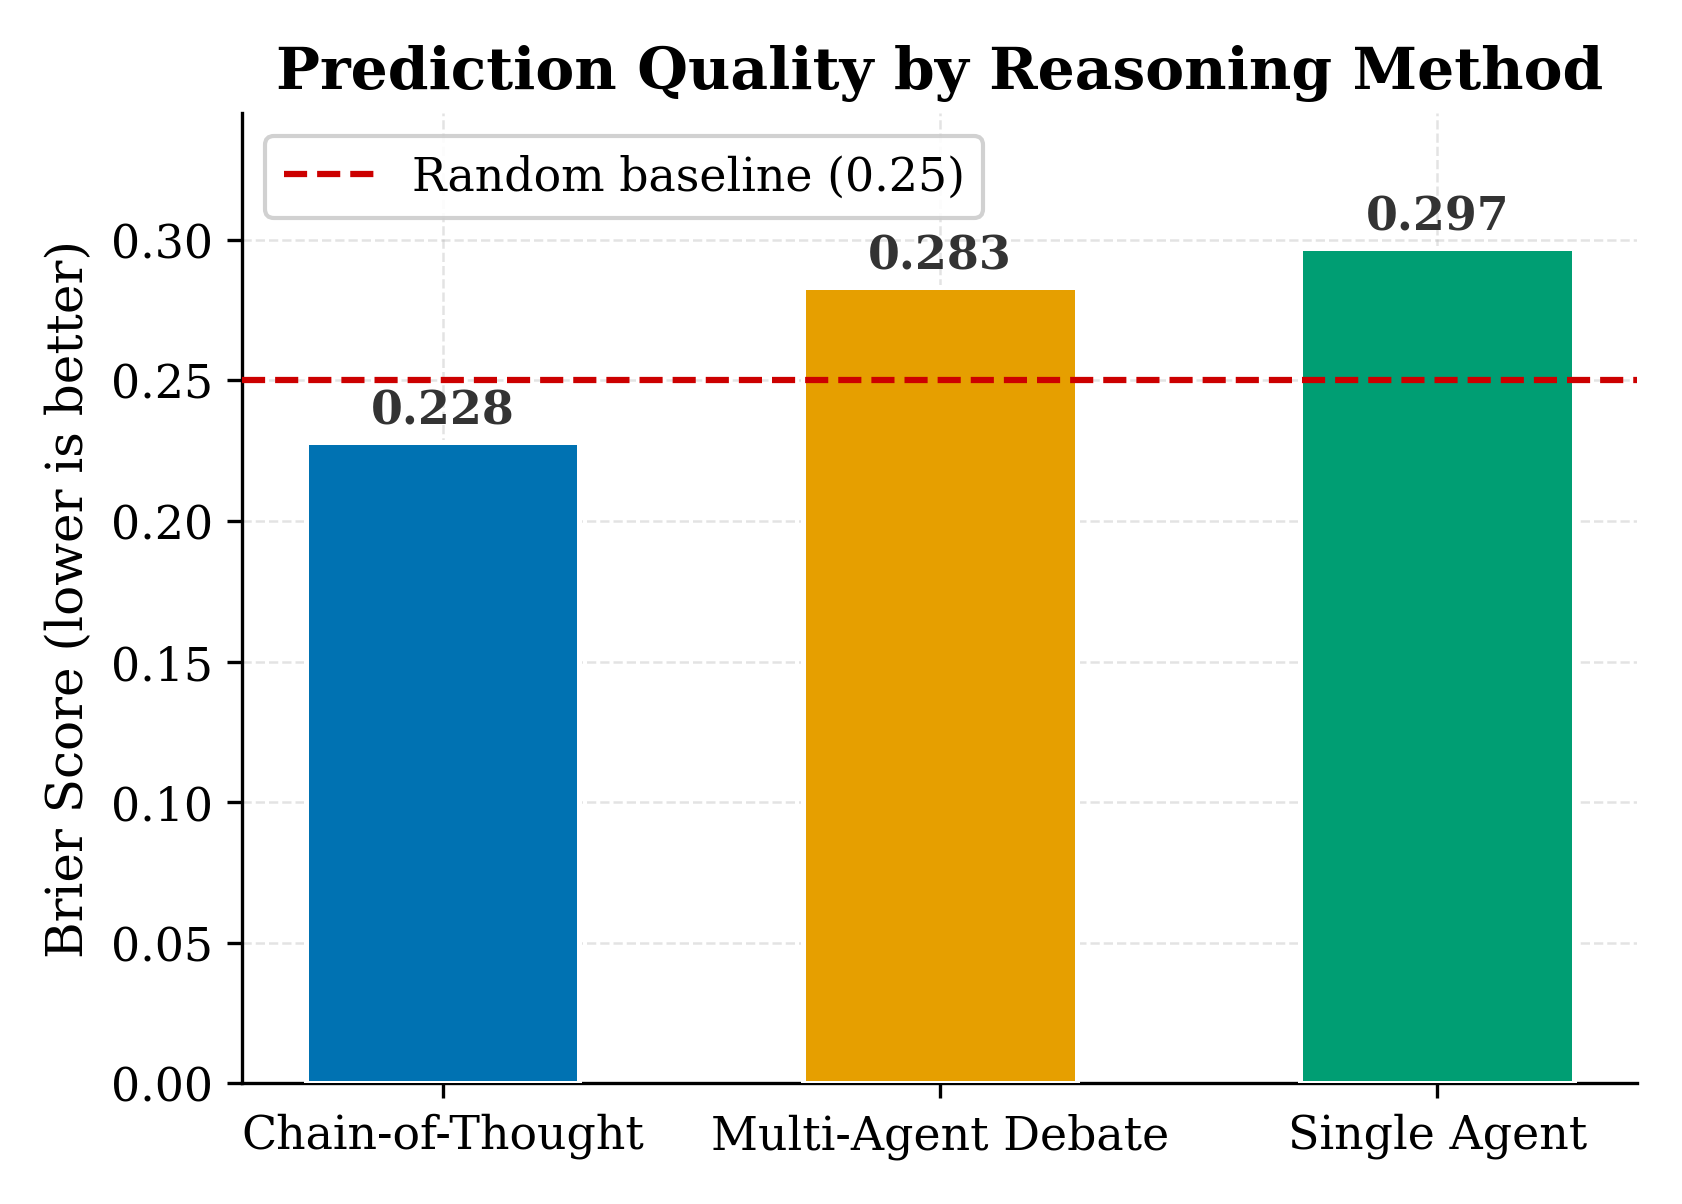
\includegraphics[width=0.72\textwidth]{fig_brier_bar.png}
\caption{Brier score comparison across the three reasoning methods. Lower is better. The dashed reference at 0.25 represents a 50/50 random predictor. Chain-of-thought (CoT) is the only method that beats the random baseline. Multi-agent debate and single agent both fall above 0.25, indicating performance below random on probabilistic accuracy.}
\label{fig:brier}
\end{figure}

\begin{figure}[H]
\centering
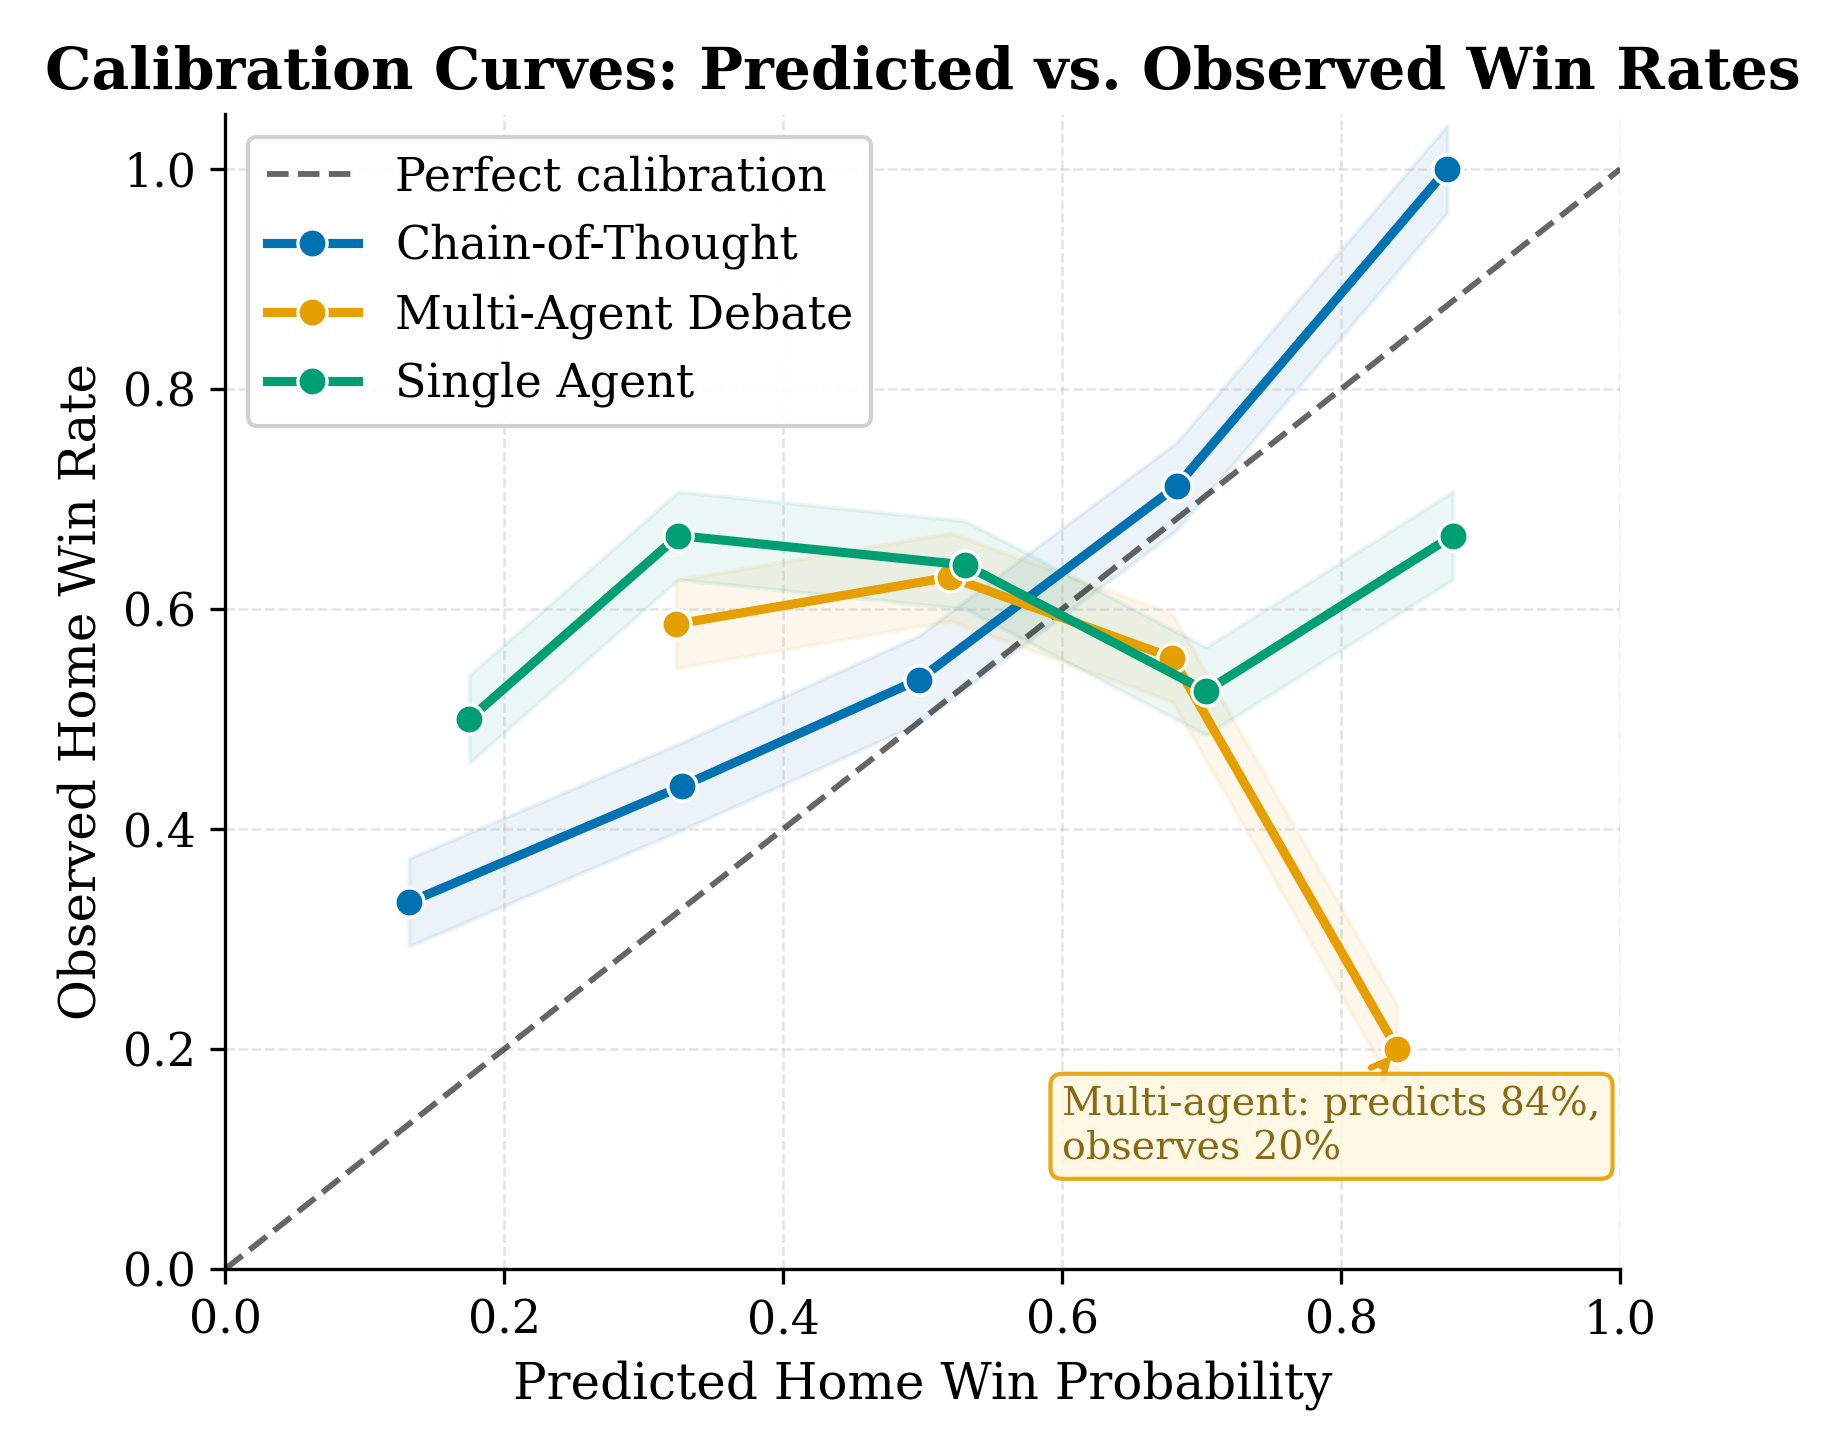
\includegraphics[width=0.82\textwidth]{fig_calibration.png}
\caption{Calibration curves for all three methods. The dashed diagonal represents perfect calibration. CoT (blue) tracks closely to the diagonal in the 0.4--0.8 range. Multi-agent debate (orange) diverges sharply at high confidence: when it predicts 80--100\% home-win probability, the actual home-win rate drops to 20\%, indicating dangerous overconfidence when agents converge. Single agent (green) is systematically miscalibrated across all bins.}
\label{fig:calibration}
\end{figure}

\begin{figure}[H]
\centering
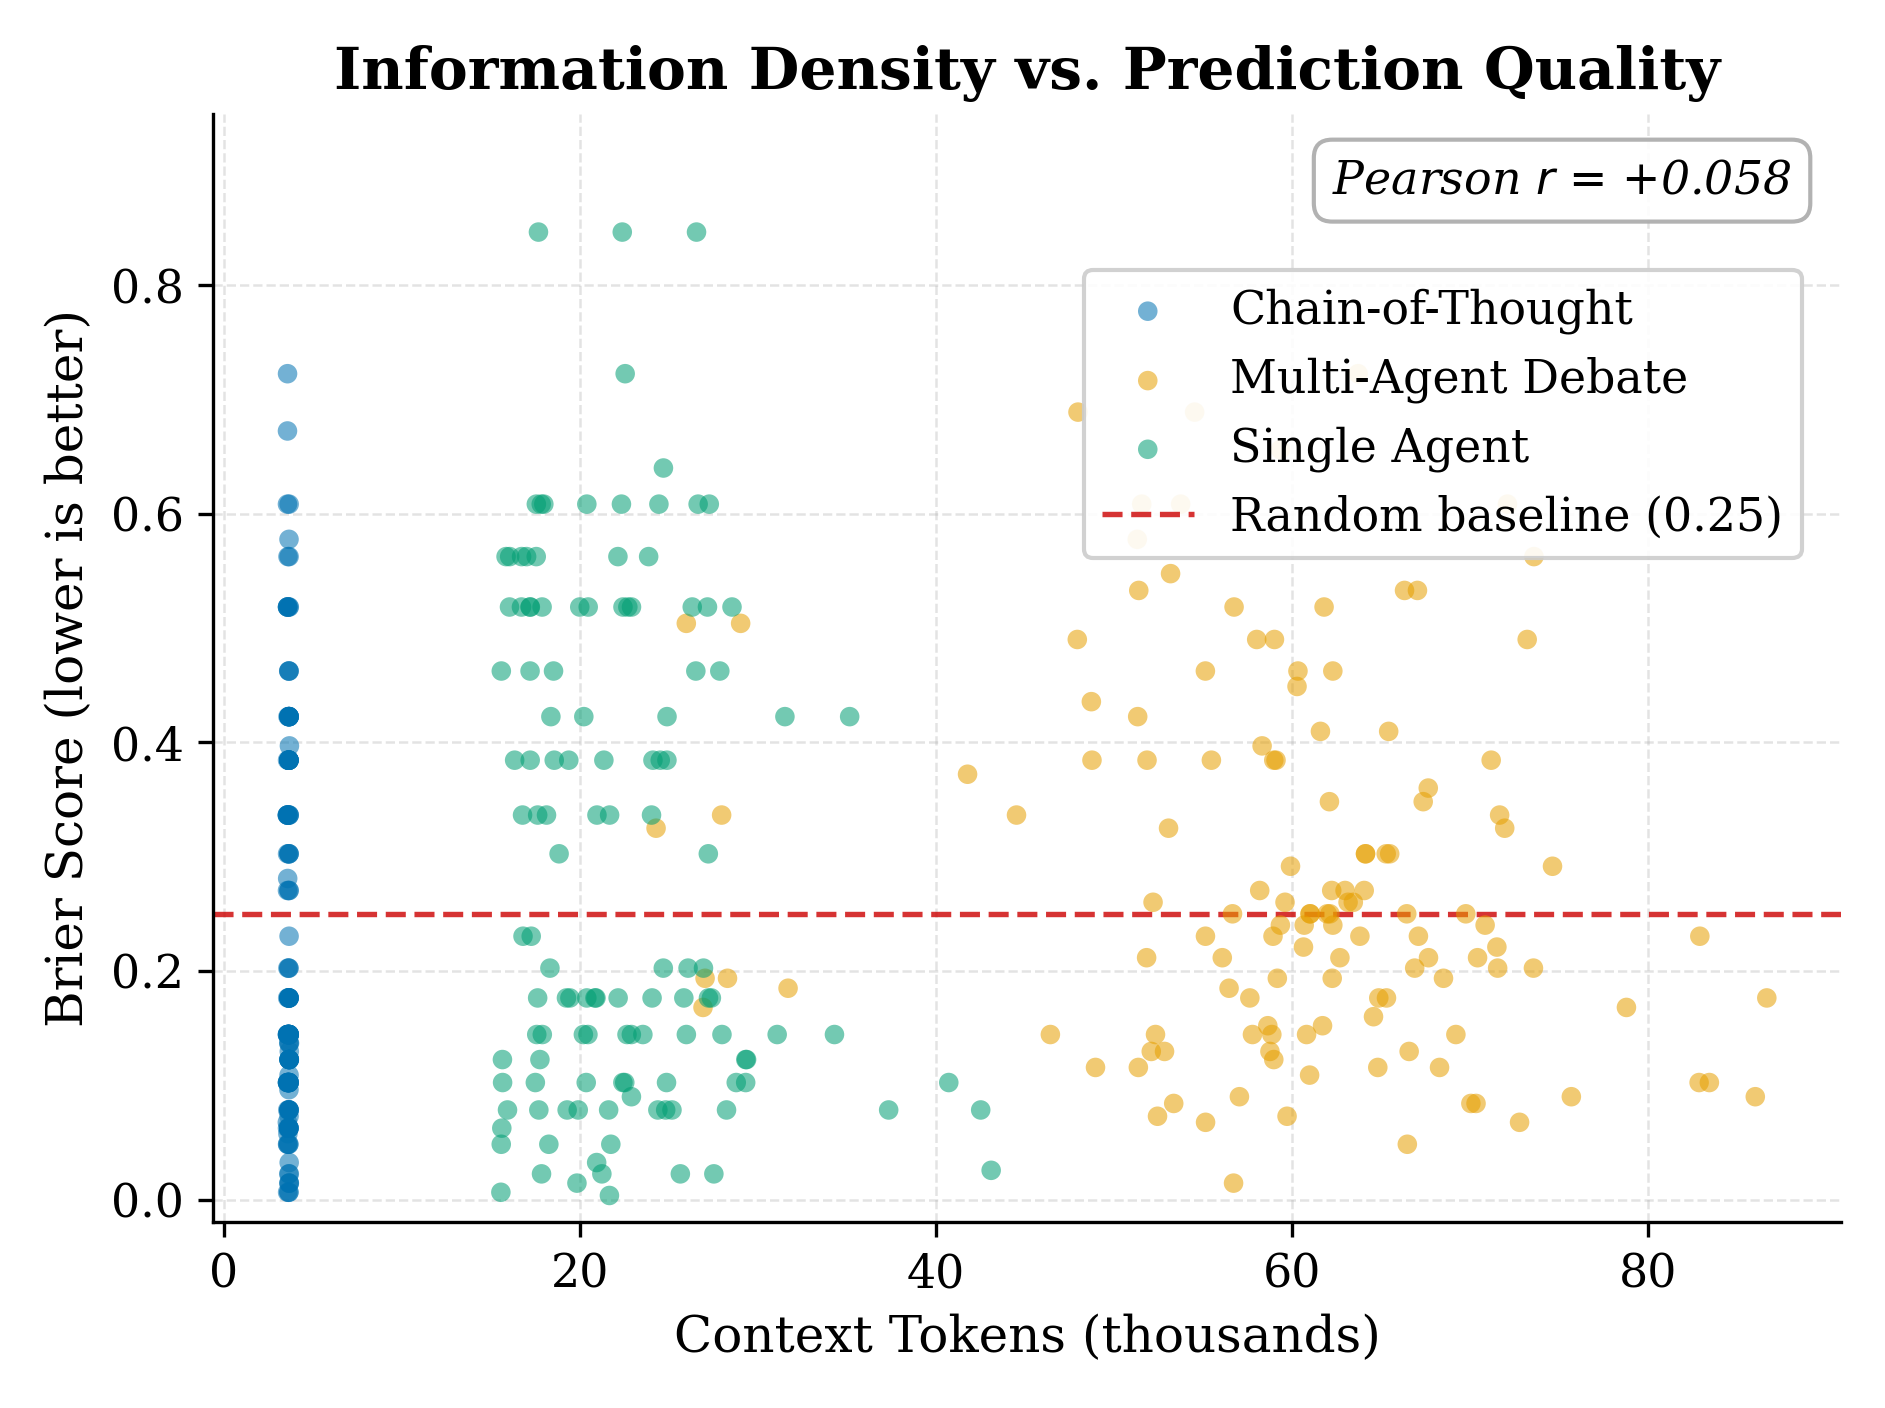
\includegraphics[width=0.82\textwidth]{fig_density.png}
\caption{Information density (context tokens) versus Brier score for all 389 game-method predictions. CoT predictions (green, left cluster) use far fewer tokens since evidence is gathered via Python calls with no intermediate LLM context. Multi-agent debate (gold, right cluster) uses 3--5$\times$ more tokens due to three agents debating across two rounds. The Pearson $r = +0.058$ indicates a weak positive relationship: games with more available context are marginally harder to predict, consistent with more-covered games having tighter and harder-to-exploit betting lines.}
\label{fig:density}
\end{figure}

\begin{figure}[H]
\centering
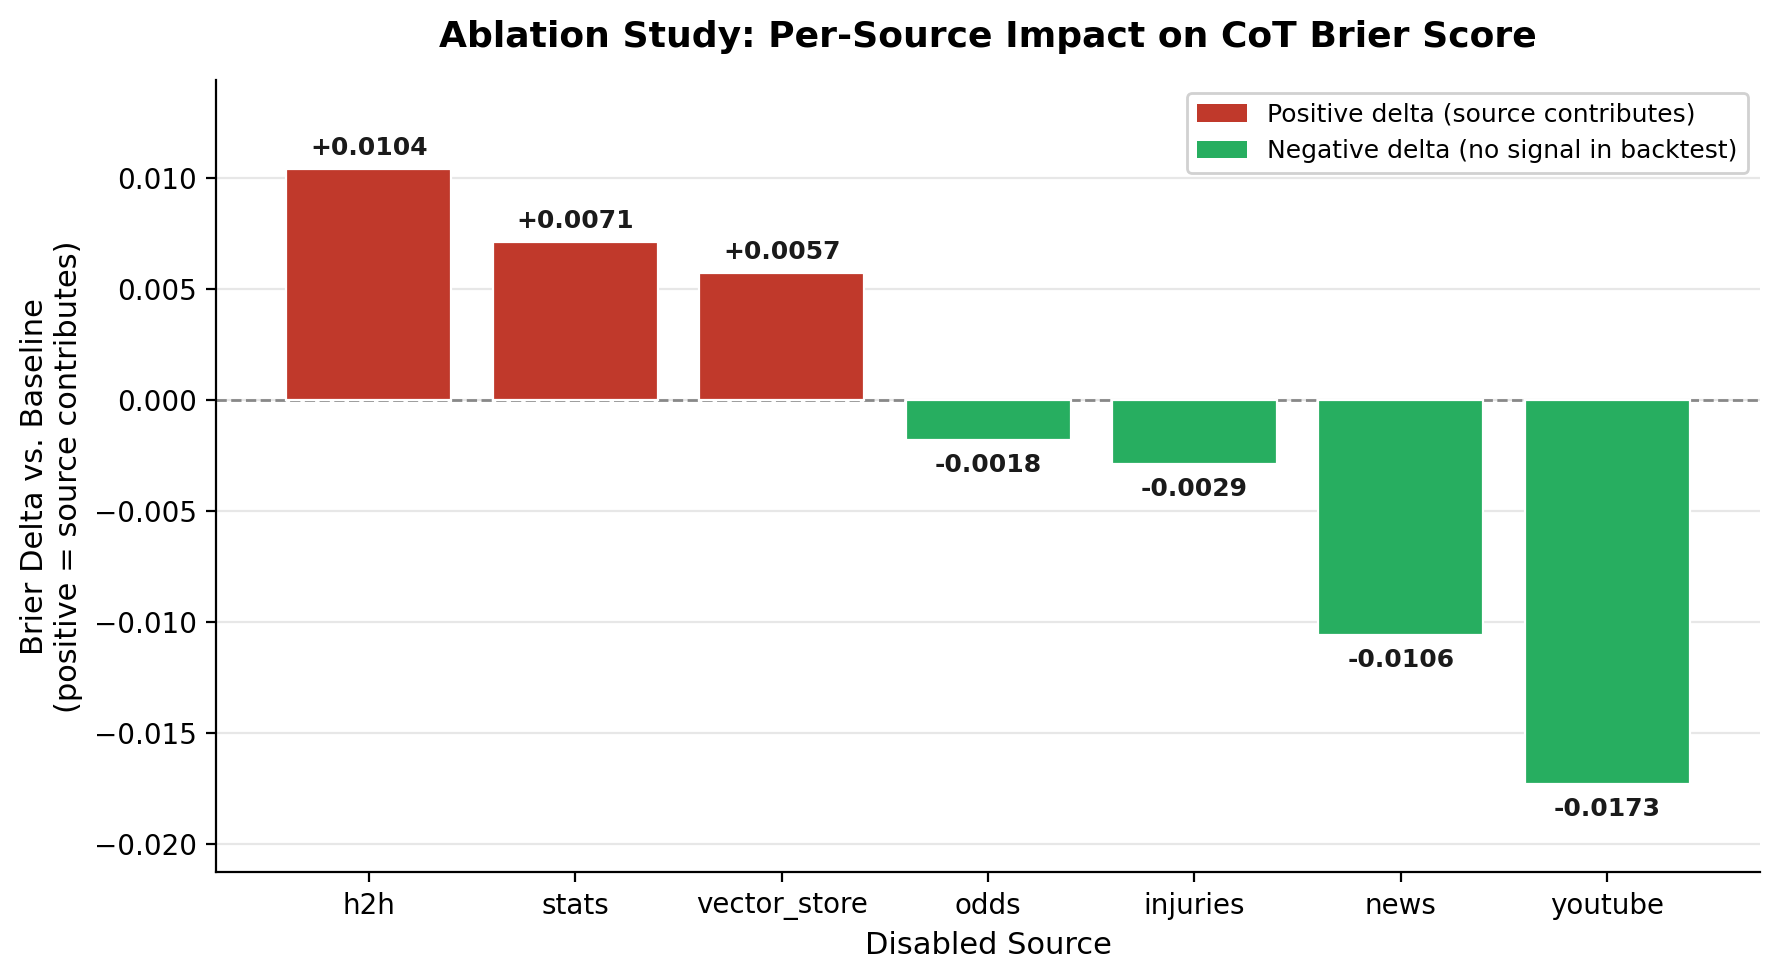
\includegraphics[width=0.82\textwidth]{fig_ablation.png}
\caption{Per-source ablation results. Each bar shows the change in CoT Brier score when that source is disabled (positive delta means the source contributes; negative means it adds no signal in the backtest). Head-to-head records (h2h, $+0.010$), team stats ($+0.007$), and the ChromaDB vector store ($+0.006$) are the three sources with real historical data and all show positive deltas. The four sources on the right (odds, injuries, news, YouTube) return no historical snapshots for past games; their near-zero or negative deltas reflect sampling noise rather than genuine information value.}
\label{fig:ablation}
\end{figure}

\end{document}
